\documentclass[11pt,answers]{exam}
\usepackage{listings}
\usepackage{pdfsync}

%
%  Created by Mike Helmick on 2006-09-13.
%  Copyright (c) 2006 Mike Helmick. All rights reserved.
%
%

\newif\ifpdf
\ifx\pdfoutput\undefined
\pdffalse % we are not running PDFLaTeX
\else
\pdfoutput=1 % we are running PDFLaTeX
\pdftrue
\fi

\ifpdf
\usepackage{subfigure}
\usepackage[pdftex]{graphicx}
\else
\usepackage{graphicx}
\fi

% exam settings
%\boxedpoints
%\pointsinmargin
%\printanswers 
\noprintanswers

\usepackage{color} 
\definecolor{SolutionColor}{rgb}{0.8,0.9,0.9} 
\shadedsolutions 


%
%  Update these values for running headers
%
\firstpageheader{\bf\Large CSA174}{\bf\Large FINAL EXAM - Part 2}{\bf\Large
  2007-12-11 }
\runningheader{CSA 174 FINAL EXAM}{Miami University}{Part 2}
\addpoints

\begin{document}

\begin{center} 
  \fbox{\fbox{\parbox{5.5in}{\centering
    CSA174 - Fall 2007 - Final Exam \newline
	Miami University \newline
	\newline
	There are 105 possible points on this exam.\newline
	Your grade will be calculated out of 100 points.\newline
 	In this part there are \numquestions\  questions for a total of  \numpoints\ points.
}}}
\end{center} 

% setup standard options for the including code fragments
\lstset{language=Java,numbers=left, numberstyle=\tiny, stepnumber=1, numbersep=5pt, showstringspaces=true}

\vspace{0.1in} 
\hbox to \textwidth{Name:\enspace\hrulefill} 
\hbox to \textwidth{Instructor/Section:\enspace\hrulefill} 

\section*{Instructions}
\begin{itemize}
 \item This exam is being administered in two parts - the scantron type answer section and programming questions
 \item This exam is closed book - you may have 1 piece of 8.5” x 11” paper that you have prepared in advance.
 \item No electronic devices may be used during the exam: this includes calculators, iPods, PDAs, and cellular phones. 
 \item You have 120 minutes (2 hours and 0 minutes) to complete BOTH sections of the exam. 
\end{itemize}

\section*{In this booklet}
\begin{enumerate}
	\item {\bf Write your name, section, instructor at the top of this page.}
	\item {\bf Mark all answers for these questions in this booklet.}
	\item {\bf Please use accurate Java syntax to receive full credit.}
\end{enumerate}	

\section*{Form Number}
\begin{center}
	\fbox{\fbox{\parbox{5.5in}{\centering
	{\huge{{\bf This is part 2 of the exam:\newline
	  Programming Questions}}}
	}}}
\end{center}

\newpage

% Questions start here:
\begin{questions}
\section*{Programming Questions}

\question[11] The {\tt StringUtils} class is incomplete, complete these methods.
\begin{parts}
 \part The method {\tt swapFirstAndLast} should swap the first and last elements of the {\tt String} array argument.  If the array was fewer than two (2) elements, it should do nothing.  Write the code for this method:
 \part The method {\tt randomWordOfTheDay} should return a random word in the array.   It should be possible to obtain any of the words in the array.   If the {\tt wordList} is empty, return {\tt ""}.
\end{parts}

\begin{verbatim}
import java.util.Random;
public class StringUtils {
    public static void swapFirstAndLast( String[] words ) {
\end{verbatim}

\begin{solution}[2in]
\end{solution}

\begin{verbatim}		
    } 
	
    public static String randomWordOfTheDay( String[] wordList ) {
\end{verbatim}

\begin{solution}[2.5in]
\end{solution}

\begin{verbatim}	
    }	
}	
\end{verbatim}

\newpage
\question[12] Suppose that a Car class has been defined.  One of its methods is {\tt getMileage()} which returns an {\tt int} indicating the number of miles the {\tt Car} has been driven.  Another {\tt Car} method is a {\tt void} method named {\tt setPrice()} whose only parameter is a {\tt double}, indicating the price at which that car should be sold.  Suppose that {\tt parkingLot} is an two-dimensional array of {\tt Cars} that has already been declared and filled with {\tt Car} objects.
\par
Write code below that will set the price of all cars in {\tt parkingLot}  as follows: If the car’s mileage is below 10,000, the price should be \$10,000.  Cars whose mileage is at least 10,000, but less than 50,000 should have a price of \$8,000.  All other cars should be sold for \$5,000.

\begin{verbatim}
public class CarDealer {

    public static void main( String[] args ) {
        Car[][] parkingLot = PlaceWhereCarsComeFrom.getCarArray();
        // BEGIN ANSWER
\end{verbatim}

\begin{solution}[4.5in]
\end{solution}

\begin{verbatim}
        // END ANSWER
    }
}	
\end{verbatim}
 
\newpage

\question[13] Complete the following Java class as specified.  The {\tt Person} class represents a person, some information about them, and their location on the map.   The {\tt Location} class is defined here.
\begin{lstlisting}
public class Location {
	private int x_pos;
	private int y_pos;
	
	public Location( int x, int y ) {
		x_pos = x;
		y_pos = y;
	}
	
	public void setX( int x ) {
		x_pos = x;
	}
	
	public void setY( int y ) {
		y_pos = y;
	}
}	
\end{lstlisting}

The {\tt Person} class is defined starting here, you will need to refer to the Location class for some of the methods.   Look for the word {\bf TODO} to indicate methods that need to be completed
 
\begin{verbatim}
public class Person {
    private String name;
    private int age; 
    private Location location;

    // TODO: write the person constructor that initialize all of the fields
    public Person( String name, int age, int xLoc, int yLoc ) {
        // BEGIN ANSWER
\end{verbatim}
\begin{solution}[2in]
	
\end{solution}
\begin{verbatim}
        // END ANSWER
    }
\end{verbatim}
\newpage

\begin{verbatim}
	// TODO: Create a constructor that initializes the person's name and age
	// The location should be set to a default of (5,5)
    public Person( String name, int age ) {
        // BEGIN ANSWER
\end{verbatim}
\begin{solution}[2in]	
\end{solution}

\begin{verbatim}
        // END ANSWER
    }

    // TODO: return the distance of this person (their locaiton)
    // to the origin (0,0)
\end{verbatim}
\hspace{.4in}Distance formula: $\sqrt{ (x_2 - x_1)^2 + (y_2 - y_1)^2 }$
\begin{verbatim}
    public double distanceToOrigin() {
       // BEGIN ANSWER
\end{verbatim}
\begin{solution}[3in]
\end{solution}

\begin{verbatim}
        // END ANSWER
    }

}
\end{verbatim}

\newpage
\question[14] An integer array can be used to store the population of cities arranged on a stretch of highway. Cities are considered crowded if:

\begin{enumerate}
	\item It and its immediate neighbor have a total population of 10 or more (for the two cities on the end).  If the city is on the end, then this is the population of the city, plus the population of the only city bordering it.
	\item It and its immediate neighbors have a total population of 15 or more (for the cities in the interior).   A city's population, plus the population of the city to the left and to the right.
\end{enumerate}
\par
Write the body of the method below that accepts an integer array (length $>=$ 2), representing the population of a series of cities, and returns a boolean array indicating whether each city is considered crowded. For example, the following integer array represents the population of 9 cities.


\par Example:
\begin{figure}[h]
    \begin{center}
        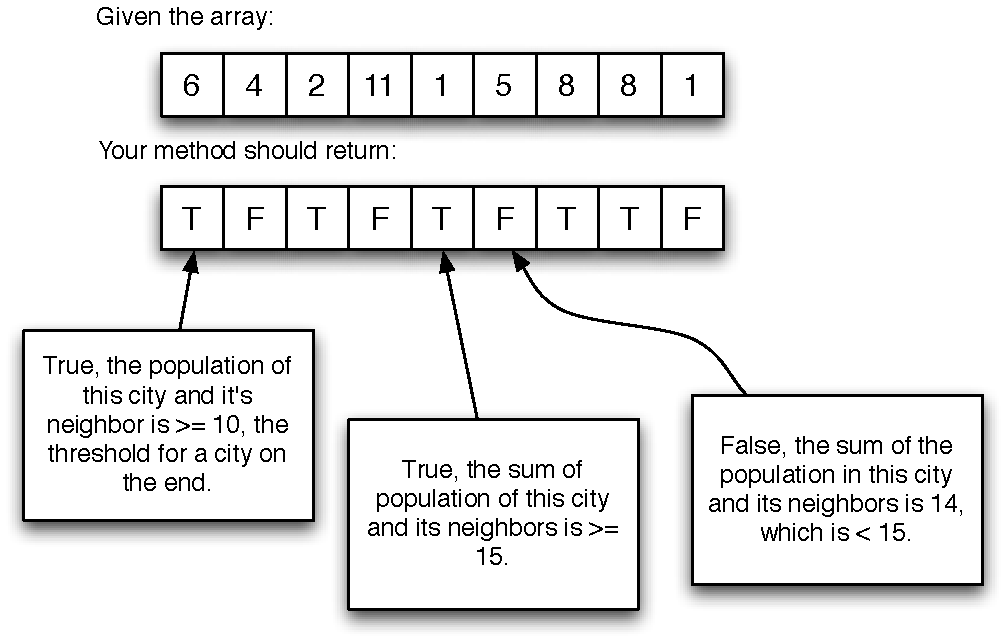
\includegraphics[width=6in]{finalExam_progQuestion_4}
    \end{center}
\end{figure}

\par Place your answer on the next page...

\newpage
\begin{verbatim}
public class Population {
    
    public static boolean[] crowded( int[] population ) {	
\end{verbatim}

\begin{solution}[6in]
\end{solution}

\begin{verbatim}
    }

}	
\end{verbatim}

\newpage

\question[5] A Niven number is a number that is exactly divisible by the sum of its digits.   The first 9 integers are obviously divisible by themselves.   After that:
\begin{itemize}
	\item 10 is a Niven number: $1 + 0 = 1 \rightarrow$, 10 is divisible by 1
	\item 11 is NOT a Niven number: $1 + 1 = 2 \rightarrow$, 11 is not divisible by 2
	\item 12 is a Niven number: $1 + 2 = 3 \rightarrow$, 12 is divisible by 3
\end{itemize}
For reference, here are the Niven numbers through 40 \newline
{\tt 1, 2, 3, 4, 5, 6, 7, 8, 9, 10, 12, 18, 20, 21, 24, 27, 30, 36, 40} \newline

\par
Write a static method called {\tt isNiven()} that takes in an {\tt int} value and returns a {\tt boolean}, indicating if the number passed in is a Niven number or not.  

\begin{verbatim}
public class NumberMethods {
    // BEGIN ANSWER
\end{verbatim}

\begin{solution}[5in]
\end{solution}

\begin{verbatim}
    // END ANSWER
}	
\end{verbatim}

\end{questions}

\end{document}

